\lecture{3}{Mon 9 Mar 2020 09:59}{La Diagnosi}{

La prima ipotesi in caso di episodi di comportamenti irrazionali è \textbf{l'uso di sostanze}, se non ci sono precedenti, traumi o episodi che possano spiegarlo, o premorbodità. 

\paragraph{Etichettare} le persone ha delle conseguenze anche stigmatizzanti, va evitato quando possibile.    

Il DSM nasce dopo la seconda guerra mondiale, spinto anche dall'emergenza psichiatrica data dalle guerre.
La prima rivoluzione è stata nel 1980 con il DSM III, la seconda nel V.
\begin{itemize}
	\item Stimolata dall’aumento della prevalenza di 
	\item Disturbi psichici conseguenti alla II G.M.
	\item Buona copertura dello spettro psicopatologico
	\item Descrizioni narrative dei vari disturbi
	\item Teoria psicoanalitica
	\item Scarsa affidabilità della diagnosi: 
	\item  inferire conflitti inconsci
\end{itemize}
Il primo a parlare di PSD è stato Freud, ma era concepito in termini psicodinamici.
\begin{itemize}
	\item Criteri diagnostici descrittivi ed espliciti
	\item operazionali per ogni disturbo;
	\item Abbandono della teoria psicoanalitica;
	\item Diagnosi basata su sintomi e segni;
	\item Approccio multi-assiale e politetico;
	\item Sviluppo di interviste strutturate per 
accertare la presenza dei criteri ($\uparrow$ inter-
rater reliability).
\end{itemize}

La classificazione multi-assiale consiste nel classificare i disfunzionamenti su ogni livello della persona, non soltanto a livello clinico:
\begin{itemize}
	\item Asse I: Sindromi cliniche
	\item Asse II: Disturbi di personalità e RM
	\item Asse III: Condizione medica generale
	\item Asse IV: Problemi psicosociali/ambientali
	\item Asse V: Funzionamento generale
\end{itemize}
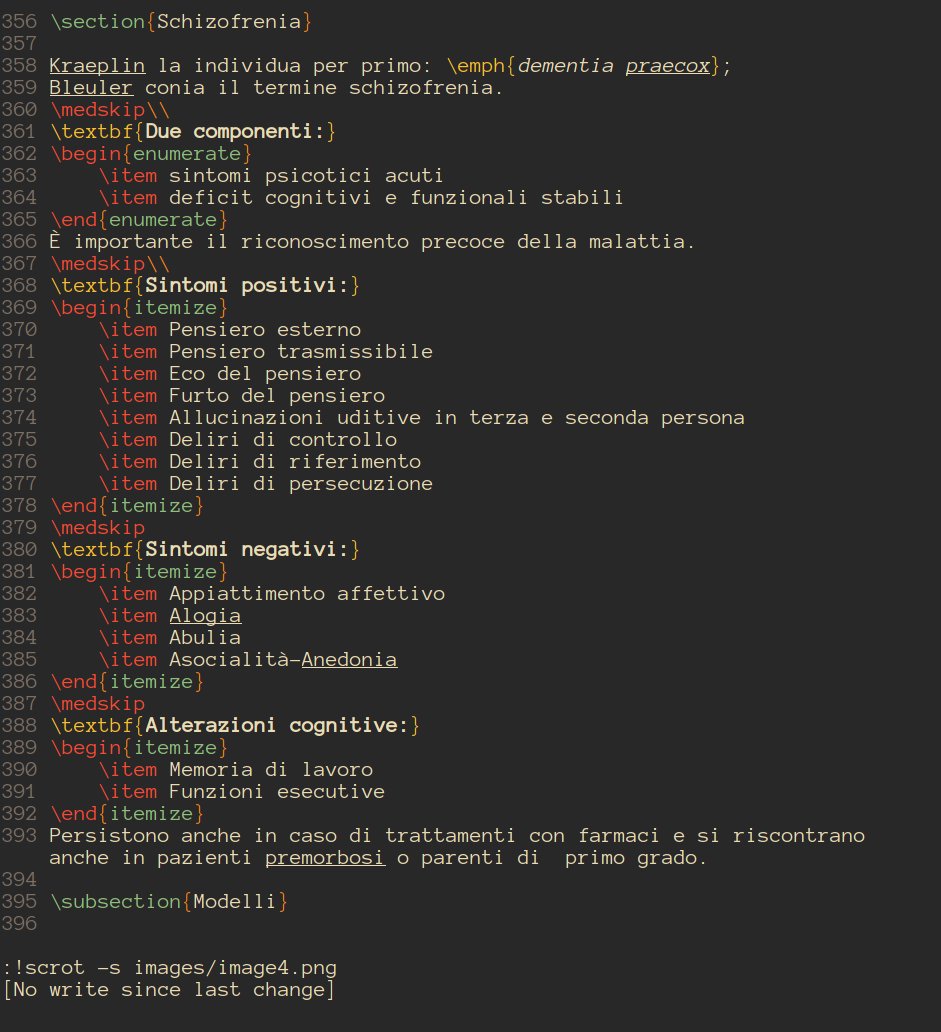
\includegraphics[width=\linewidth]{./images/image4}
\paragraph{L'approccio politetico} 
\begin{itemize}
	\item Struttura dei criteri diagnostici:
	\item (Breve descrizione del quadro clinico);
	\item Criteri sintomatologici (x di una serie di y)
	\item Criteri di esclusione
	\item Compromissione funzionale/disagio
\end{itemize}






